\documentclass{article}
\usepackage[margin=1in]{geometry}
\usepackage{setspace}
\usepackage{amsmath}
\usepackage{amssymb}
\usepackage{physics}
\usepackage{graphicx}
\usepackage{relsize}

\title{Math 132 Final}
\author{Jiaping Zeng}
\date{12/13/2020}

\begin{document}
\setstretch{1.5}

\newpage
\begin{itemize}
      \item [P2] Find and plot all $z\in\mathbb{C}$ such that $z^3=-1$.\\
            \textbf{Answer}: We have $z^3=-1\implies z^3=\cos\pi+i\sin\pi$, so by the $n$th roots formula, the roots are:\\
            $z_1=\cos\frac{\pi}{3}+i\sin\frac{\pi}{3}=\frac{1}{2}+\frac{\sqrt{3}}{2}i$\\
            $z_2=\cos(\frac{\pi}{3}+\frac{2\pi}{3})+i\sin(\frac{\pi}{3}+\frac{2\pi}{3})=-1$\\
            $z_3=\cos(\frac{\pi}{3}+\frac{4\pi}{3})+i\sin(\frac{\pi}{3}+\frac{4\pi}{3})=\frac{1}{2}-\frac{\sqrt{3}}{2}i$
            \begin{center}
                  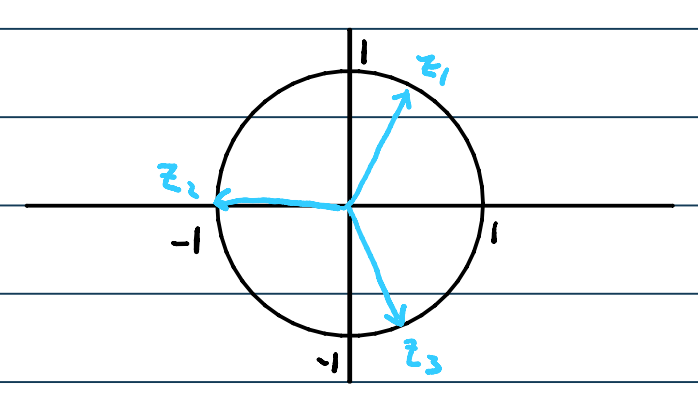
\includegraphics[width=3in]{p2.png}
            \end{center}
\end{itemize}

\newpage
I certify on my honor that I have neither given nor received any help, or used any non-permitted resources, while completing this evaluation.\\
Signature:
\includegraphics[width=2in]{signature.png}\\
Date: 12/13/2020


\end{document}